% LaTeX rebuttal letter example. 
% 
% Copyright 2019 Friedemann Zenke, zenkelab.org
%
% Based on examples by Dirk Eddelbuettel, Fran and others from 
% https://tex.stackexchange.com/questions/2317/latex-style-or-macro-for-detailed-response-to-referee-report
% 
% Licensed under cc by-sa 3.0 with attribution required.

\documentclass[11pt]{article}
\usepackage[utf8]{inputenc}
\usepackage{lipsum} % to generate some filler text
\usepackage{fullpage}
\usepackage{graphicx}
\usepackage{amsmath}

% import Eq and Section references from the main manuscript where needed
% \usepackage{xr}
% \externaldocument{manuscript}

% package needed for optional arguments
\usepackage{xifthen}
% define counters for reviewers and their points
\newcounter{reviewer}
\setcounter{reviewer}{0}
\newcounter{point}[reviewer]
\setcounter{point}{0}

% This refines the format of how the reviewer/point reference will appear.
\renewcommand{\thepoint}{\arabic{point})} 

% command declarations for reviewer points and our responses
\newcommand{\reviewersection}{\stepcounter{reviewer} \bigskip \hrule
                  \section*{Reviewer \thereviewer}}

\newenvironment{point}
   {\refstepcounter{point} \bigskip \noindent {\textbf{Referee~Point~\thepoint} } ---\ }
   {\par }

\newcommand{\shortpoint}[1]{\refstepcounter{point}  \bigskip \noindent 
	{\textbf{Reviewer~Point~\thepoint} } ---~#1\par }

\newenvironment{reply}
   {\medskip \noindent \begin{sf}\textbf{Reply}:\  }
   {\medskip \end{sf}}

\newcommand{\shortreply}[2][]{\medskip \noindent \begin{sf}\textbf{Reply}:\  #2
	\ifthenelse{\equal{#1}{}}{}{ \hfill \footnotesize (#1)}%
	\medskip \end{sf}}

\newcommand{\appropto}{\mathrel{\vcenter{
  \offinterlineskip\halign{\hfil$##$\cr
    \propto\cr\noalign{\kern2pt}\sim\cr\noalign{\kern-2pt}}}}}

\begin{document}

\section*{Response to the referee}
% General intro text goes here
We thank the referee for their critical assessment of our work. In the
following we address their concerns point by point. All changes made to the
manuscript have been boldfaced. 

% Let's start point-by-point with Reviewer 1
\hrule
% Point one description 
\begin{point}
	Since neither set of models using the two different opacity tables provide a
	good match to the properties of the Jao gap, the possibility that the
	convective kissing instability is not the correct explanation for the gap
	has to be considered.

	The first paper to offer an explanation for the existence of the gap (MacDonald
	\& Gizis 2018) states 'Convective mixing is treated as a diffusion process
	with the diffusion coefficient determined from mixing length theory.' and
	'The fully implicit nature of our code also prevents the convective kissing
	instability discovered and described by van Saders \& Pinsonneault (2012).'
	The treatment of convective mixing as a diffusion process is probably the
	reason why MacDonald \& Gizis find a single episode of convection zone
	merger (for models in which merger occurs) and hence a single dip in the
	luminosity function, which seems to be the case for the Jao gap (inferred
	from figure 1 of this paper).

	In contrast, the use of instantaneous mixing leads to multiple episodes of
	convection zone merger and this could be the reason why the authors find
	two dips in the luminosity function (inferred from their figures 7 and 8).
	The authors need to give in the paper a convincing argument as to why the
	instantaneous mixing approximation is valid, particularly as using the
	diffusion approach seems to more physically consistent with current
	understanding of turbulent mixing. This should involve estimates using
	mixing length theory of the mixing time scale at all stages of the merger,
	with special attention to mixing time scales within one mixing length on
	either side of the point of contact between the merging convection zones.
	This region is where the mixing time scale is most likely to be the
	longest.

	The mixing time scale then needs to compared to other relevant time scales
	including the time scale for deuterium to come into equilibrium and the
	time scale at which the helium-3 abundance is modified by nuclear
	reactions.

	If it turns out that the instantaneous mixing approximation is not valid, then
	there needs to be discussion of alternative approaches and their
	consequences. The thrust of the paper could be changed to show that the CKI
	is not the correct explanation of the gap.
\label{pt:timescale}
\end{point}

% Our reply
\begin{reply}
	We have carefully investigated the referee's concern relating to DSEP's
	use of an instantaneous mixing approximation. After this investigation
	we believe that instantaneous mixing is a valid approximation. The reasons
	for this are outlined below; Additionally, much of the justification has been
	include in the text of the manuscript on page 5.

	% As the referee says the primary point to clarify here is the ratio of the
	% overturn timescale to the timestep length. DSEP treats convective mixing
	% instantanously throught a single shell and we evolve models composed of
	% 5000 radial shells. Convective overturn timescales for M-dwarfs have not
	% insignifigant uncertanties on them (with different sources reporting
	% overturn times between 70 and 300 days). Therefore, for a single shell the
	% overturn timescale will be of order $10^{5}$s. However, all of these
	% estimates are order of magnitude shorter than the time steps used (which
	% bottom out at around 1 Myr). Specifically, K\"apyl\"a 2021 presents
	% hydrodynamical simulations of fully convective stars and find that the
	% overturn times are on the order of $10^{7}$s (Their Table 1). Therefore,
	% convective mixing is extremly well approximated by instantanious mixing.

	The referee's concern may be addressed in two parts. First, whether or not
	instantaneous mixing is a valid approximation for species which will not
	remain in equilibrium throughout a star (such as $^{3}He$) and second
	whether or not this approximation is valid for species which will remain in
	equilibrium (such as $^{2}H$). Put another way, we address these concerns
	for species who's lifetime is long compared to the mixing timescale and for
	species who's lifetime is short compared to the mixing timescale. 
	% due to the
	% dramatically shorter lifetimes of deuterium compared to other species
	% involved in the proton-proton chains (with PPI being the most relevant for
	% the mass ranges we are investigating here).

	To the first part of this concern, species with long lifetimes compared to
	the mixing timescales, such as $^{3}$He. Instantaneous mixing will be a
	valid approximation here if the mixing timescales are much shorter than the
	timesteps used. In order to estimate the mixing timescale we look to recent
	hydrodynamical simulations of low mass stars from K\"apyl\"a 2021 which
	estimate a mixing timescale of between $10^{7}$s and $10^{8}$s depending on
	rotational period and whether or not magnetic fields are considered (their
	Table 1). These numbers are in line with estimates using mixing length
	theory from Chabrier \& Baraffe 1997. The largest timestep allowed in the
	models we run is 50 million years, more than five orders of magnitude lager
	than the longer estimate of the mixing timescale. Moreover, we see that we are
	resolving the mixing of $^{3}He$ (Figure 2 in the manuscript) as we observe a
	smooth increase in core $^{3}He$ concentration for gap stars in our models. 

	In addition to these timescale arguments, we direct the referee to recent
	work conducted by the MESA collaboration (Jermyn et al. 2022 Figure 2).
	MESA has recently implemented time dependent convection (TDC) in addition
	to standard mixing length theory (MLT) making use of instantaneous mixing.
	The models presented in Figures \ref{fig:MESA1} and \ref{fig:MESA2}
	(private communication with Aaron Dotter) are for stars within the Jao Gap
	(identified in MESA in Mansfield \& Kroupa 2021). Note the extreme
	similarity between the instantaneous approximation and the time dependent
	convective models.

	\begin{figure}
		\centering
		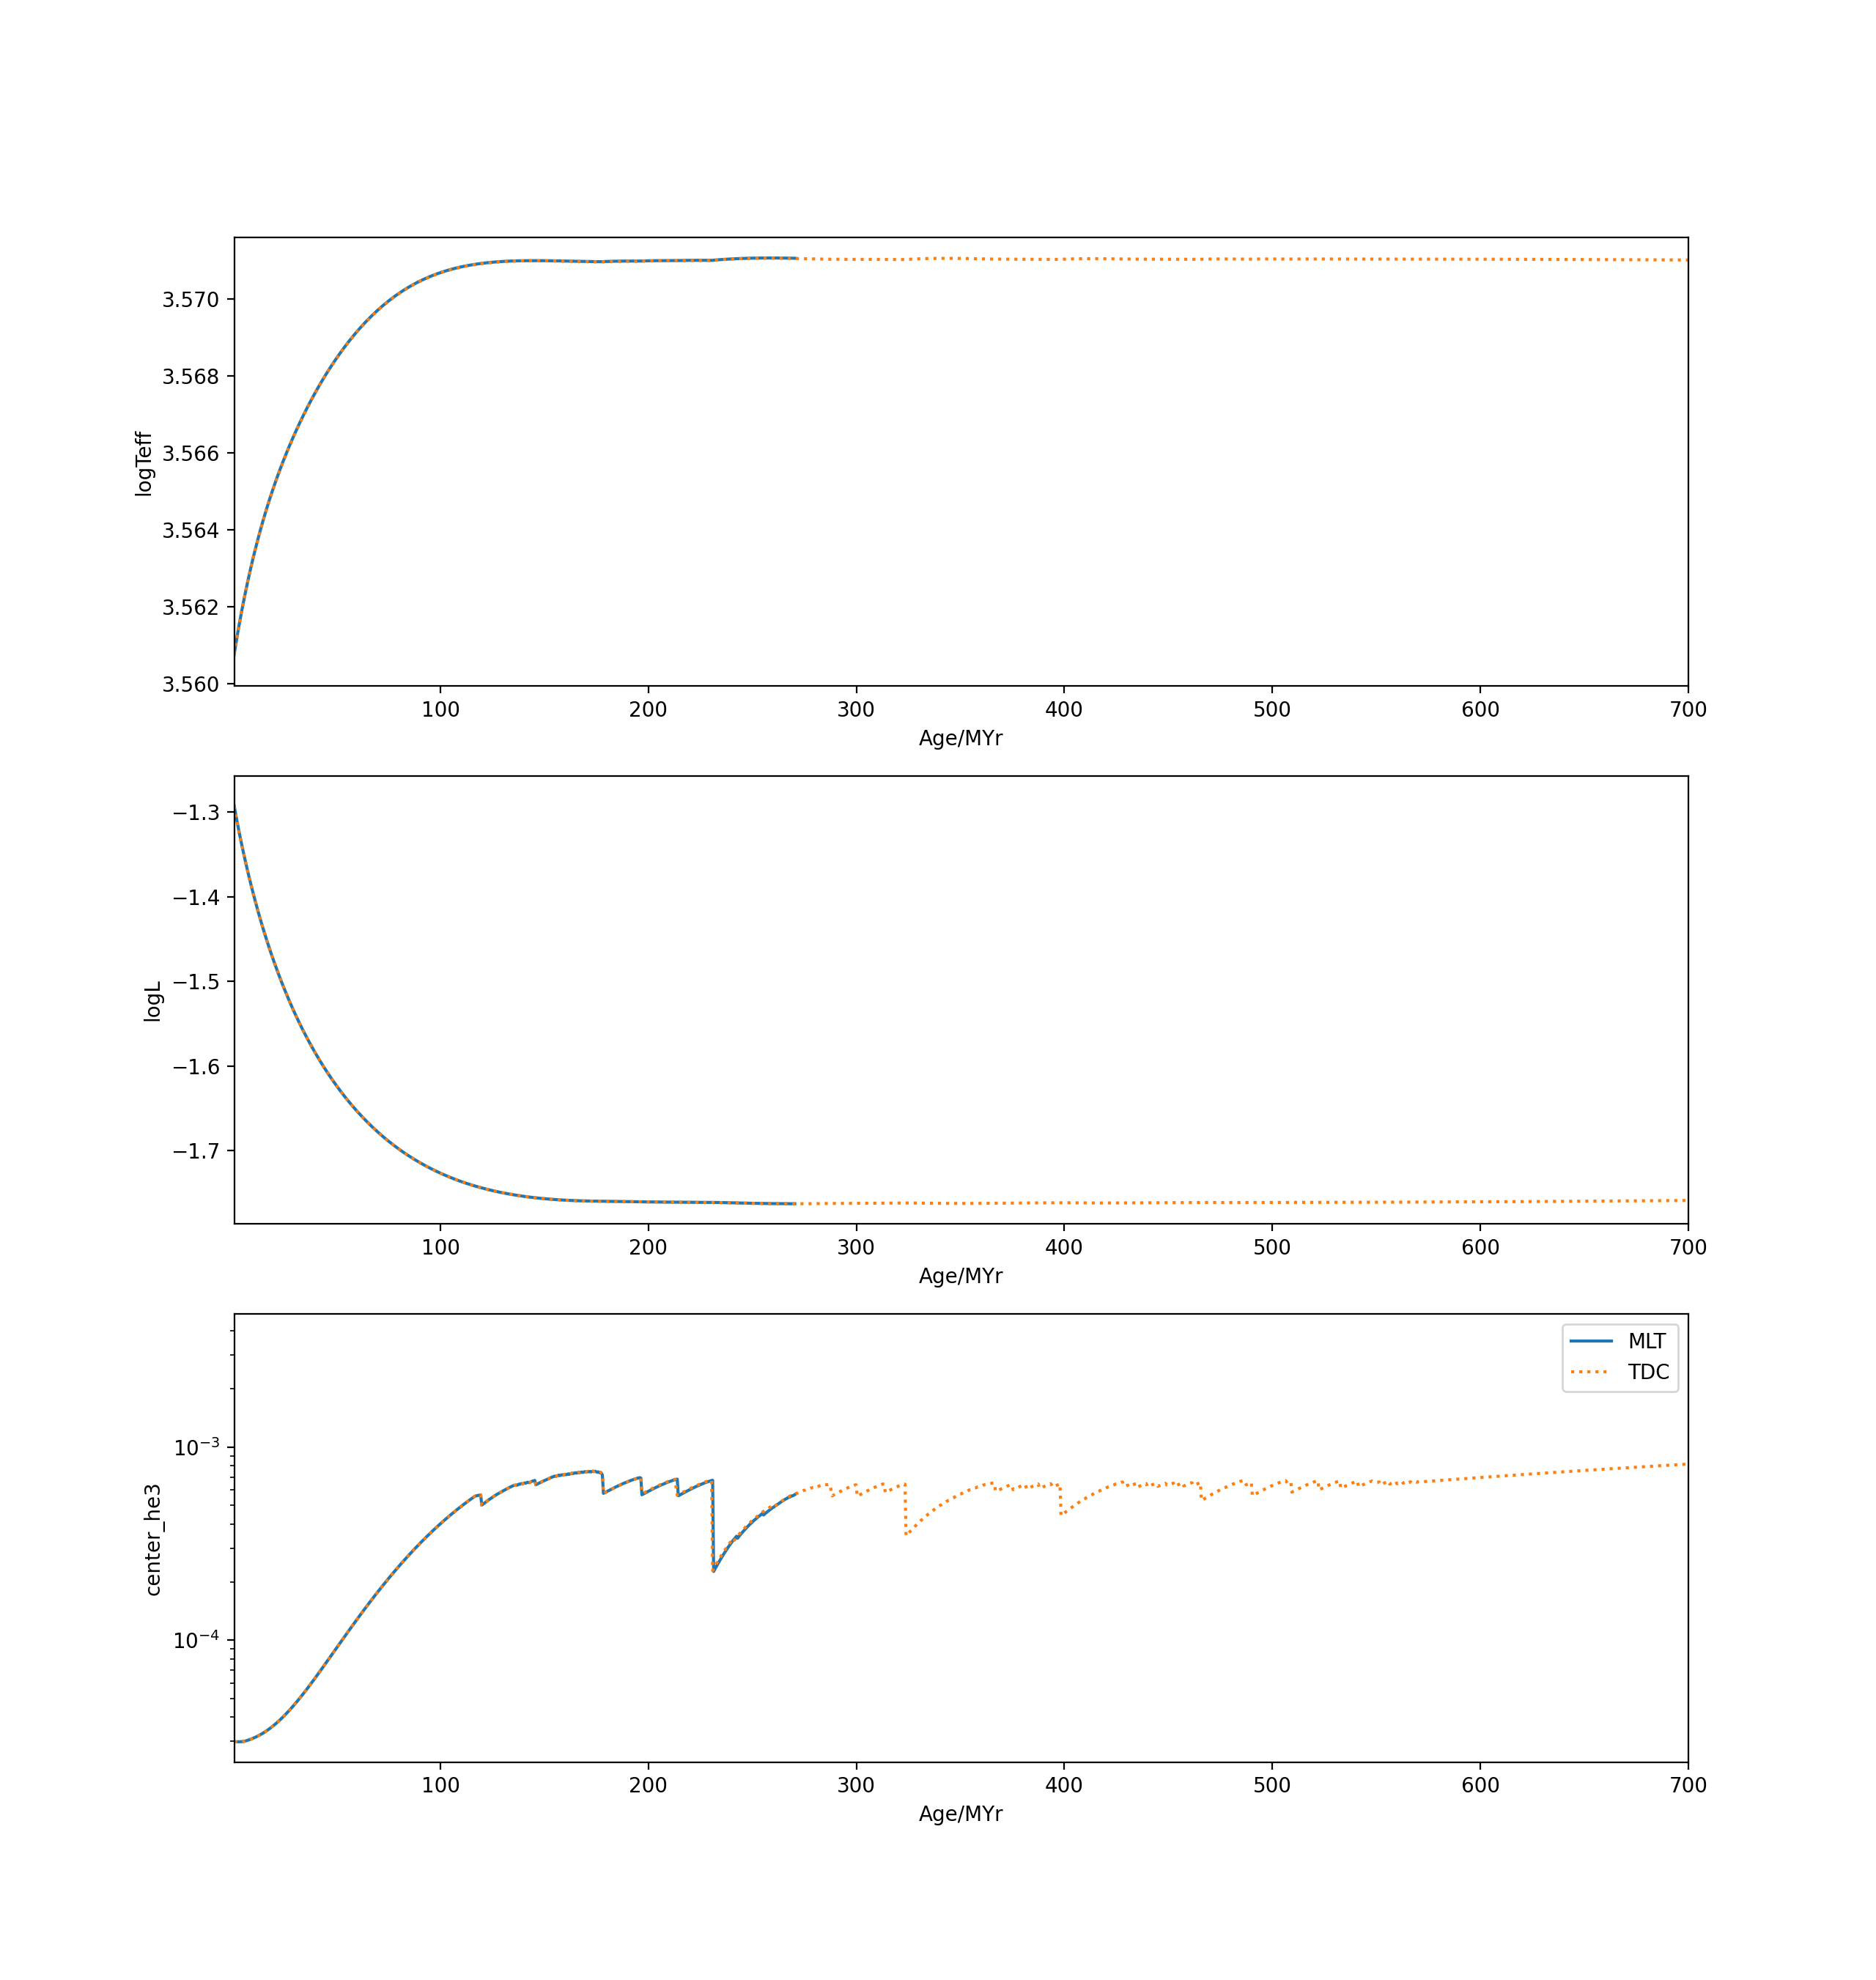
\includegraphics[width=0.85\textwidth]{./Figure_4.png}
		\caption{Results acquired through private communication with Aaron Dotter showing
		MESA models from Mansfield \& Kroupa 2021 (a model near the Jao Gap). One
		model makes use of a standard instantaneous mixing approximation while the other
		uses the newly introduced Time Dependent Convection. Note the similarity between the
		models}
		\label{fig:MESA1}
	\end{figure}
	\begin{figure}
		\centering
		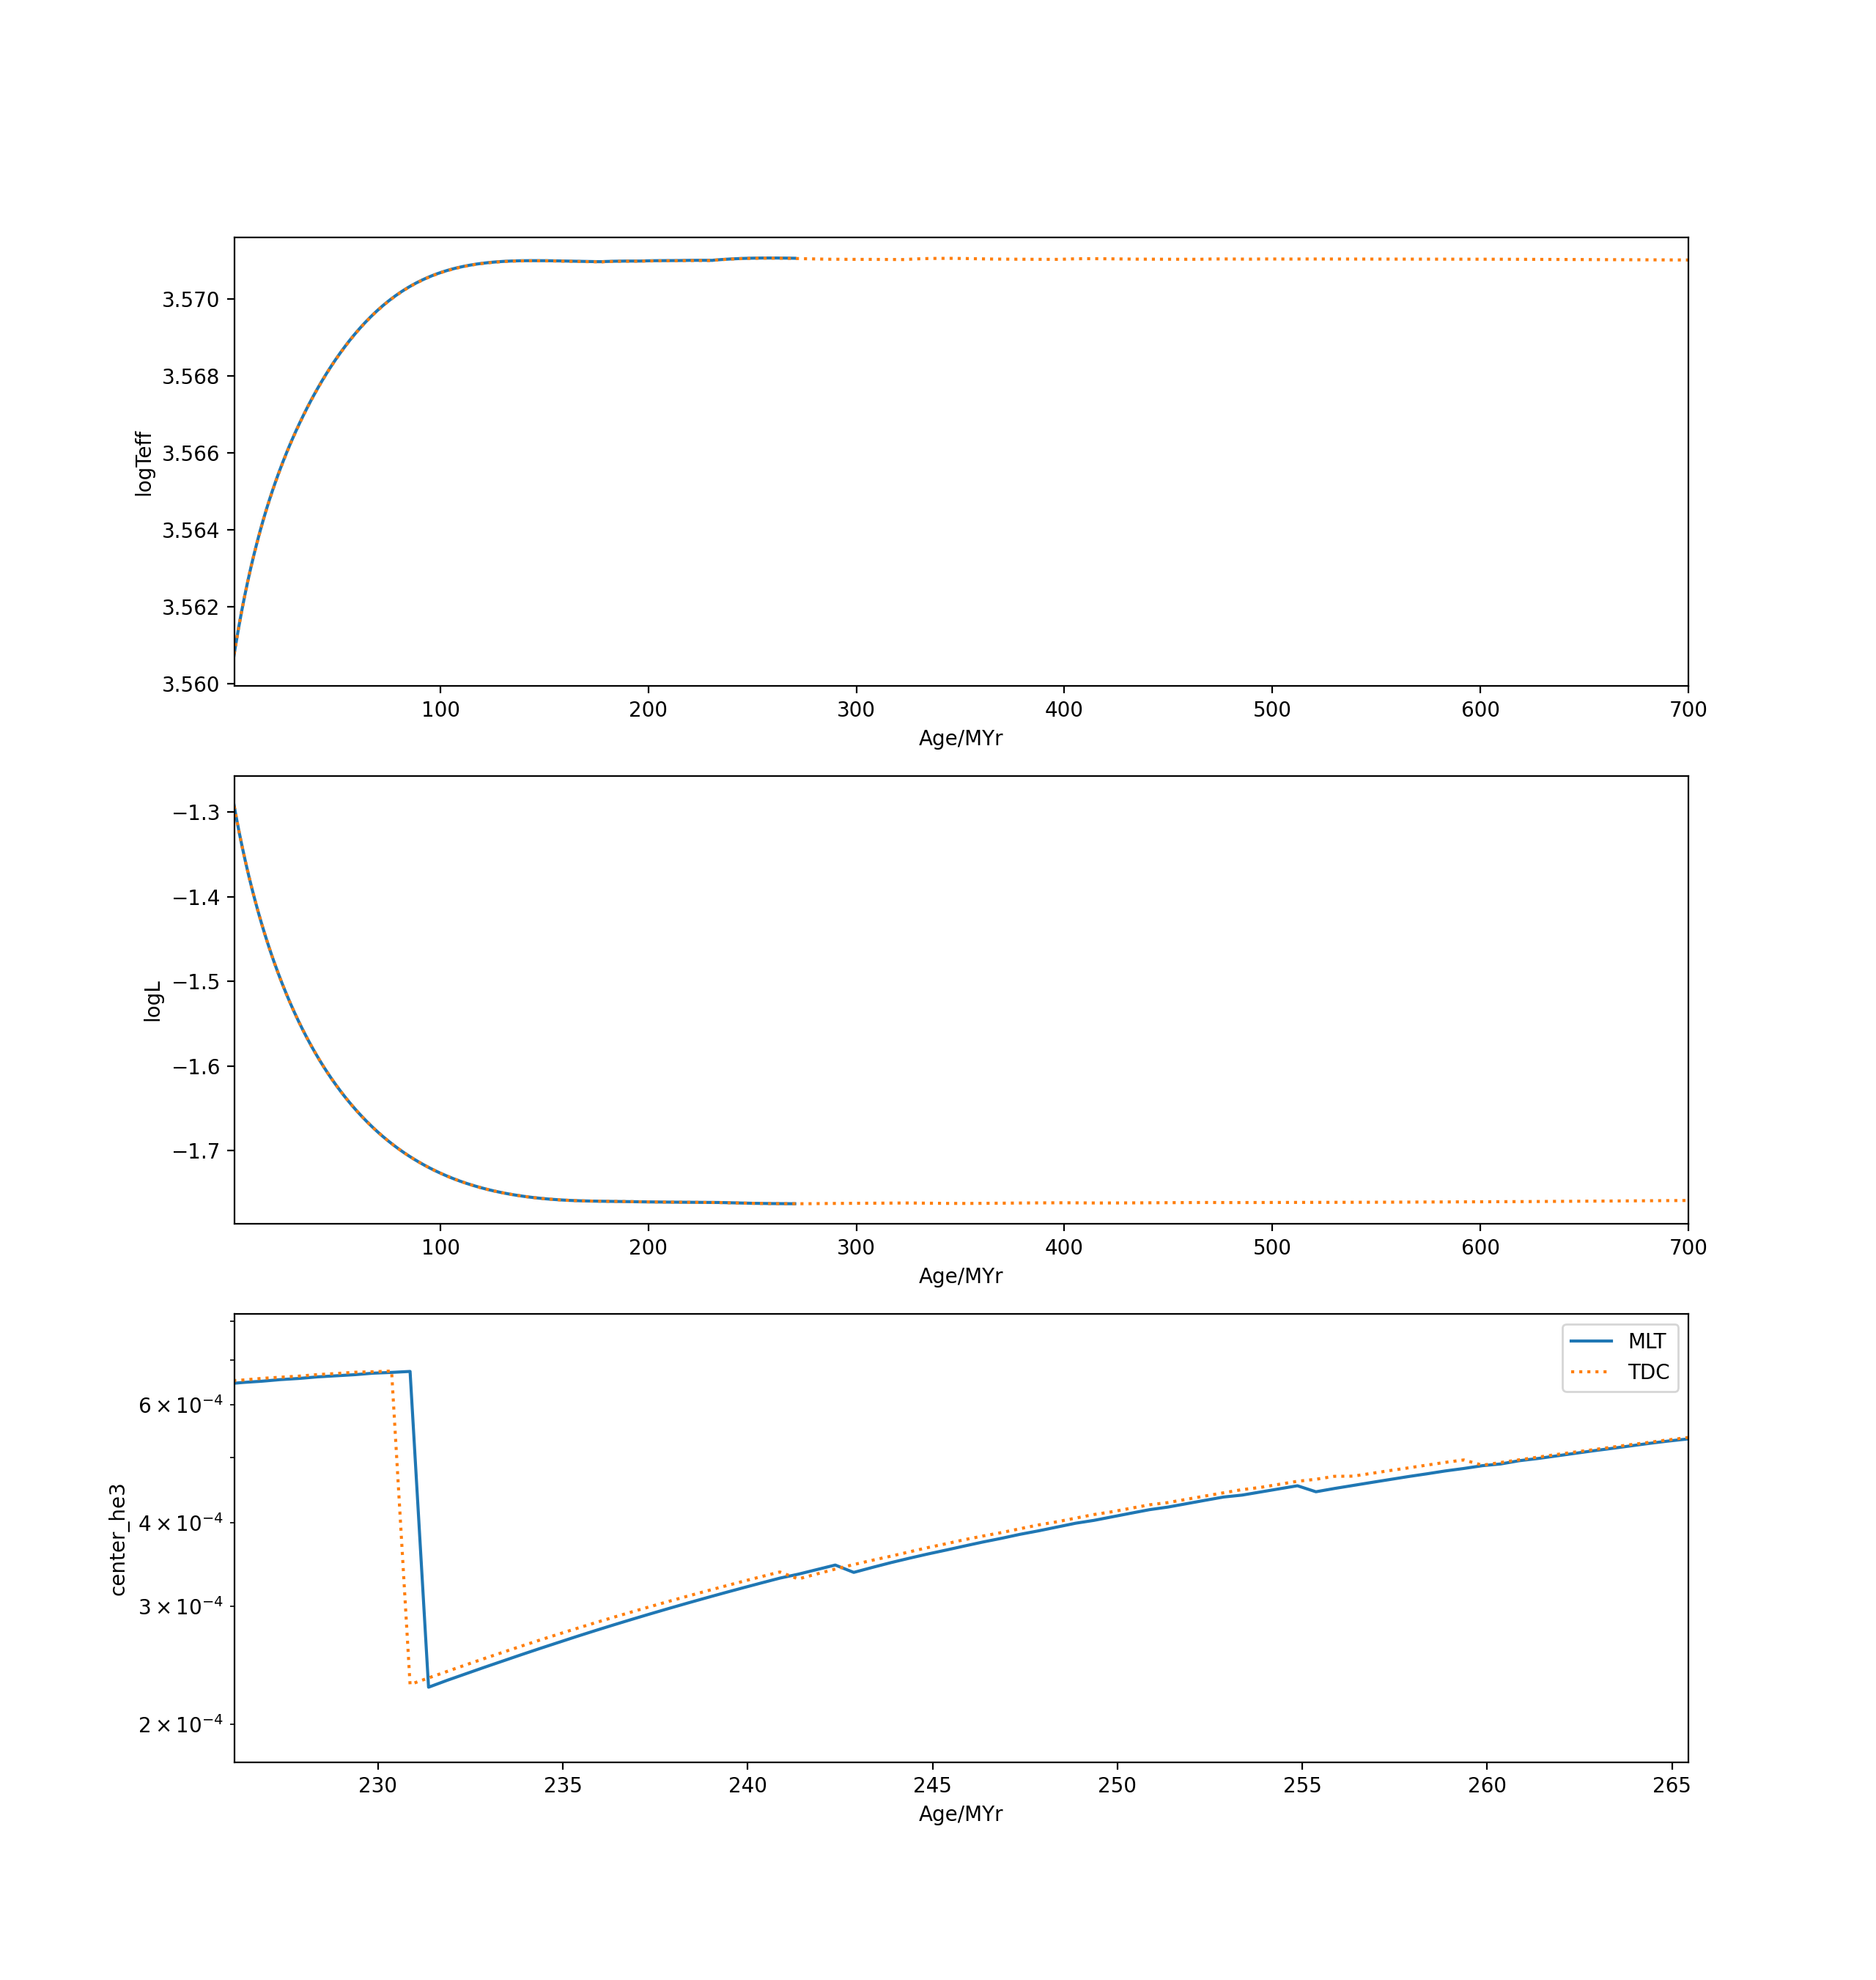
\includegraphics[width=0.85\textwidth]{./Figure_4_zoom.png}
		\caption{Results acquired through private communication with Aaron Dotter showing
		MESA models from Mansfield \& Kroupa 2021 (a model near the Jao Gap). One
		model makes use of a standard instantaneous mixing approximation while the other
		uses the newly introduced Time Dependent Convection. Note the similarity between the
		models}
		\label{fig:MESA2}
	\end{figure}

	A complication to this argument arises with $^{2}H$ however. The deuterium
	lifetime against proton capture is extremely short, at $10^{7}$K around
	100s. Chabrier \& Baraffe 1997 identify that an instantaneous mixing model
	of convection may have a strong suppressing effect on a models luminosity
	(20\%  at 0.1 M$_{\odot}$ and 56\% at 0.075 M$_{\odot}$). The root cause of
	this effect is identified as the build up of a deuterium gradient in a
	models core when the mixing timescale is significantly longer than the
	deuterium burning timescale. However, because the lifetime of deuterium
	against proton capture so much shorter than the lifetimes other species in
	the proton-proton 1 chain it's will remain in equilibrium with $^{1}H$. Specifically, the
	equilibrium abundance of deuterium is given by Equation \ref{eqn:2Habun}
	(where $N$ denotes the number fraction of some species and $\lambda$
	denotes reaction rates between two species).

	\begin{align}\label{eqn:2Habun}
		N_{^{2}H} \rightarrow \frac{N_{^{1}H}\lambda_{^{1}H,^{1}H}}{2\lambda(^{1}H,^{2}H)}
	\end{align}

	DSEP computes nuclear energy generation using John Bahcall's nuclear reaction
	subroutine (\texttt{exportenergy.f} available for review at
	\texttt{http://www.sns.ias.edu/\textasciitilde jnb/}) in each shell individually and
	therefore takes into account the correct, equilibrium, abundance of
	deuterium on a shell-by-shell basis. Therefore, the luminosity discrepancy
	identified by Chabrier \& Baraffe 1997 is implicitly accounted for in
	DSEP's handling of nuclear reactions and does not require a change in DSEP's
	treatment of convective mixing to account for.

	Finally, there is precedent for more complex structure in the observed
	color-magnitude diagram, Jao \& Feiden 2021 identify an under density below
	the Jao Gap in the EDR3 color magnitude diagram. While we do not have
	sufficient observational constraints or uncertainty constraints to claim
	that this under density is in fact a second gap as we find in our models it
	is not unprecedented that there may be more than one gap. Aside from this
	additional feature, one potential explanation for why there is only one gap
	that has been consistently identified in observations is that the
	population synthesis code we use does not account for age and composition
	differences within a population, all of which will act to smear multiple
	mixing events together over gigayear time-spans. We point the referee to work by
	Feiden et al. 2020, also using DSEP, which accounts for age variation within a
	population and the composition differences which are coupled to that. These
	modeling efforts also only identify a single population suggesting that the
	simplicity of our population synthesis code is in fact the root cause of
	the multiple mixing events we see in the synthetic CMD.

	Therefore, after careful investigation, we believe that our use of an
	instantaneous mixing approximation is valid.

\end{reply}

\begin{point}
	The convective mixing method used by MacDonald \& Gizis needs to be properly
	described along with the resulting differences from using instantaneous
	mixing.
	\label{pt:address}
\end{point}

\begin{reply}
	Additional text has been added to page 2 the manuscript addressing the results of
	MacDonald \& Gizis. 
\end{reply}

\begin{point}
	On line 184, the authors say that the OPLIB tables were created to resolve the
	discrepancy between helioseismic and solar model predictions of chemical
	abundances in the Sun. I find this to be an odd way to phrase the problem.
	Presumably the authors are referring to the difficulty of making solar
	models that match the sound speed profile (or almost equivalently the depth
	of the surface convection zone) determined by helioseismology given the
	composition constraints provided by the then recent new measurements of the
	surface abundances, notably the oxygen abundance. The authors should
	rephrase the problem and also discuss whether using OPLIB opacities help
	resolve the problem or not.
	\label{pt:seismo}
\end{point}

\begin{reply}
	We agree with the referee that the invocation of helioseismic discrepancies
	is confusing. Because this is not a helioseismic paper we drop from the
	text, instead just mentioning that the OPLIB tables make use of the most up
	to date physics, which is the most relevant point to our work. We do note
	here though that the OPLIB opacities did not serve to resolve any
	discrepancies.
\end{reply}

\begin{point}
	The distinction between low temperature and high temperature opacity sources
	made in the paragraph beginning on line 196 is somewhat artificial.
	Presumably the transition between low temperature and high temperature
	opacity is chosen to be between $10^{4.3}$ and $10^{4.5}$ K because there
	is where the Ferguson et al. opacities and OPAL opacities are close to each
	other. Perhaps the evolution could be affected if a different temperature
	range for the transition is used. The authors should stress in this section
	that as far as modeling the gap the main impact of using different
	opacities is on the radiative zone, and give the temperature and R (or
	density) ranges that are relevant to the radiative zone(s) so that the
	reader can see from figure 3 the expected change in opacity, and also if
	log R = -1.5 is truly a representative value in the radiative zone.

	Also, from figure 3, it seems that the OPLIB opacities are lower than the OPAL
	opacities for temperatures greater than $10^{5.5}$ K and not $10^{5}$ K as
	stated in the figure caption and also on line 203.
	\label{pt:lowtempboundary}
\end{point}

\begin{reply}
	The range where DSEP ramps from low temperature to high temperature
	opacities is determined by the temperature range where molecules can start
	to form. It is important for the low temperature opacities to be the only
	opacity source by the time the first molecules start forming. We choose to
	ramp the opacity source so that there is not a hard discontinuity. This
	same ramp has been used as standard in all DSEP models since 2008, see
	Dotter et al. 2008 for further details.

	We have updated references in our paper to Log(R)=-1.5 as a good
	approximation throughout a star. For a GS98 solar composition 1 solar mass
	model this is a good approximation; however, we calculate Log(R) throughout
	a 0.356 solar mass model (the same model used to generate Figure 2 in the
	manuscript) and find that a more representative value of Log(R) is -0.79.
	It is not surprising that this value is somewhat larger given the lower
	mass of this model and the commensurately lower pressures and temperatures.
	We have updated Figure 3 to show the opacity at Log(R) = -0.5 (-0.79 is not
	on the R grid we use).

	The referee is correct that we had mislabeled the $\log(T)$ value where
	OPLIB opacities are systematically lower than OPAL opacities. We have
	changed this to the correct value (5.2 for R=-0.5). We thank the referee
	for identifying this issue.
\end{reply}

\begin{point}
	In section 3.2, mention is made of the solar surface Z/X ratio but the actual
	value is not given. Is it the value recently determined by Magg et al.
	(2022), Z/X = 0.0225 or some other earlier value? The authors should state
	the actual Z/X value used.

	Also, the authors need to say whether or not they include gravitational
	settling and element diffusion in their solar modeling, and if they do, say
	how it is done (e.g. are elements grouped or treated independently). The
	authors should also include discussion of how well their solar models
	replicate the sound speed profile determined from helioseismology.
	\label{pt:ZX}
\end{point}

\begin{reply}
	The Z/X reference (GS98) and value have been added into the text in section 3.2 along
	with clarification that we do include gravitational settling with elements
	grouped together.

	A full discussion of the discrepancies between helioseismology and solar
	modeling is worth a second paper by itself and has been extensively
	discussion the literature so we feel this is outside the scope
	of this paper.
\end{reply}

\begin{point}
	Presumably, the authors use their solar calibrated models to set the mixing
	length ratio and initial abundances for their calculations of the evolution
	of models of low mass stars. Do they use primordial or present-day solar
	abundances? Why should the mixing length ratio be the same as the solar
	calibrated? There is evidence that the mixing length varies with stellar
	properties (e.g. Trampedach et al. 2014; Joyce \& Chaboyer 2018). A better
	fit to the location of the gap might be obtained by adjusting the mixing
	length ratio. The authors need to address these questions.
	\label{pt:alpha}
\end{point}

\begin{reply}
	The referee raises a important issue which has lead us to investigate the 
	effects of mixing length on the Jao Gap.

	We use GS98 solar abundances (Grevesse \& Sauval 1998) for all models. While, as the
	referee says, there is substantial evidence of a metallicity dependence
	for the mixing length parameter this dependence has only been calibrated
	for higher mass stars. In order to fully address this point we have run an
	additional grid of models with the mixing length parameter dramatically
	lowered ($\alpha_{ML} = 1.5$ \& $\alpha_{ML} = 1.0$). Results of that grid
	are shown in Figures \ref{fig:alphaMLML}, \ref{fig:alphaMLCMD}, and \ref{fig:alphaMLLoc}. 

	What is clear from these additional grids is that the Jao Gap location is
	sensitive to the value of the mixing length parameter with the magnitude of
	the gap being inversely proportional too the mixing length parameter
	($G_{mag} \appropto -0.15\alpha_{ML}$). Moreover, dramatically lowering the
	mixing length parameter to $\alpha_{ML} = 1.0$ does bring the location of
	the Jap Gap we model in closer agreement with the empirically measured
	location of the Gap.

	However, there is no a priori reason which we are aware of to expect the
	mixing length parameter to be so much lower in these low mass stars than it
	would be in the sun. Much of the work calling into question the use of
	solar calibrated mixing lengths in higher mass stars has identified a
	[Fe/H] dependence. Given that the population of stars which the Jao Gap has
	been identified in is relatively similar to the sun in composition
	extrapolating the empirical calibrations backward would not predict such a
	large dip in the mixing length.

	Therefore, we have modified the manuscript to include a limited discussion
	of the perils of using solar calibrated mixing length parameters, along
	with the results of our $\alpha_{ML} = 1.5$ and $1.0$ populations. Finally,
	we have added into the conclusions a call for further work to be done
	studying the Jao Gap location as a potential calibration point for the
	mixing length of lower mass stars.

	We thank the referee for pointing us in this direction.

	\begin{figure}
		\centering
		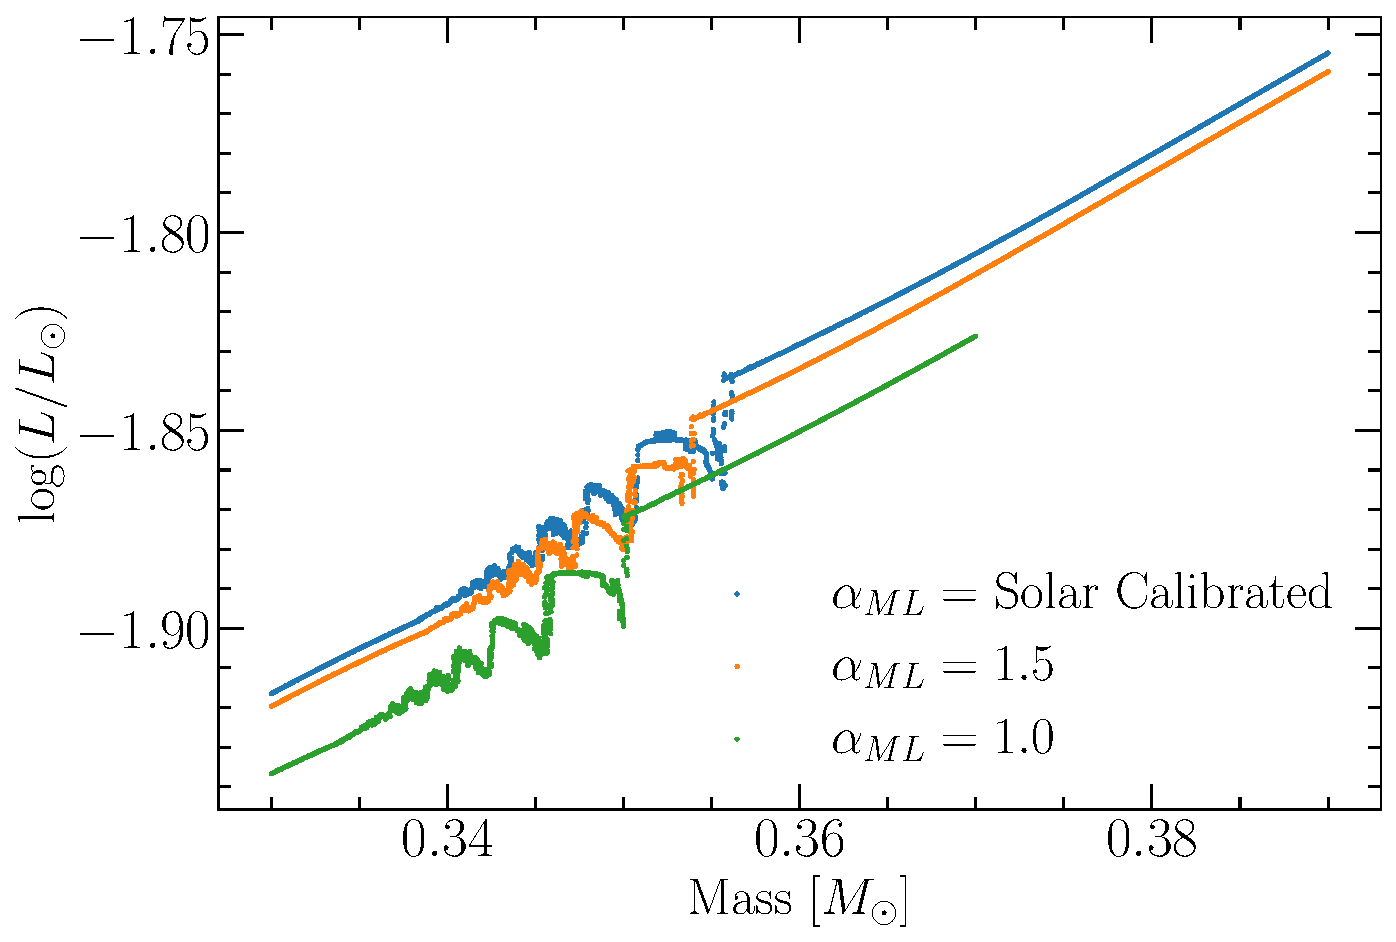
\includegraphics[width=0.8\textwidth]{./AlphaMLMassLum.pdf}
		\caption{Mass Luminosity relation for mixing length grid. From top to
		bottom: solar calibrated mixing length, mixing length of 1.5, and
		mixing length of 1.0}
		\label{fig:alphaMLML}
	\end{figure}
	\begin{figure}
		\centering
		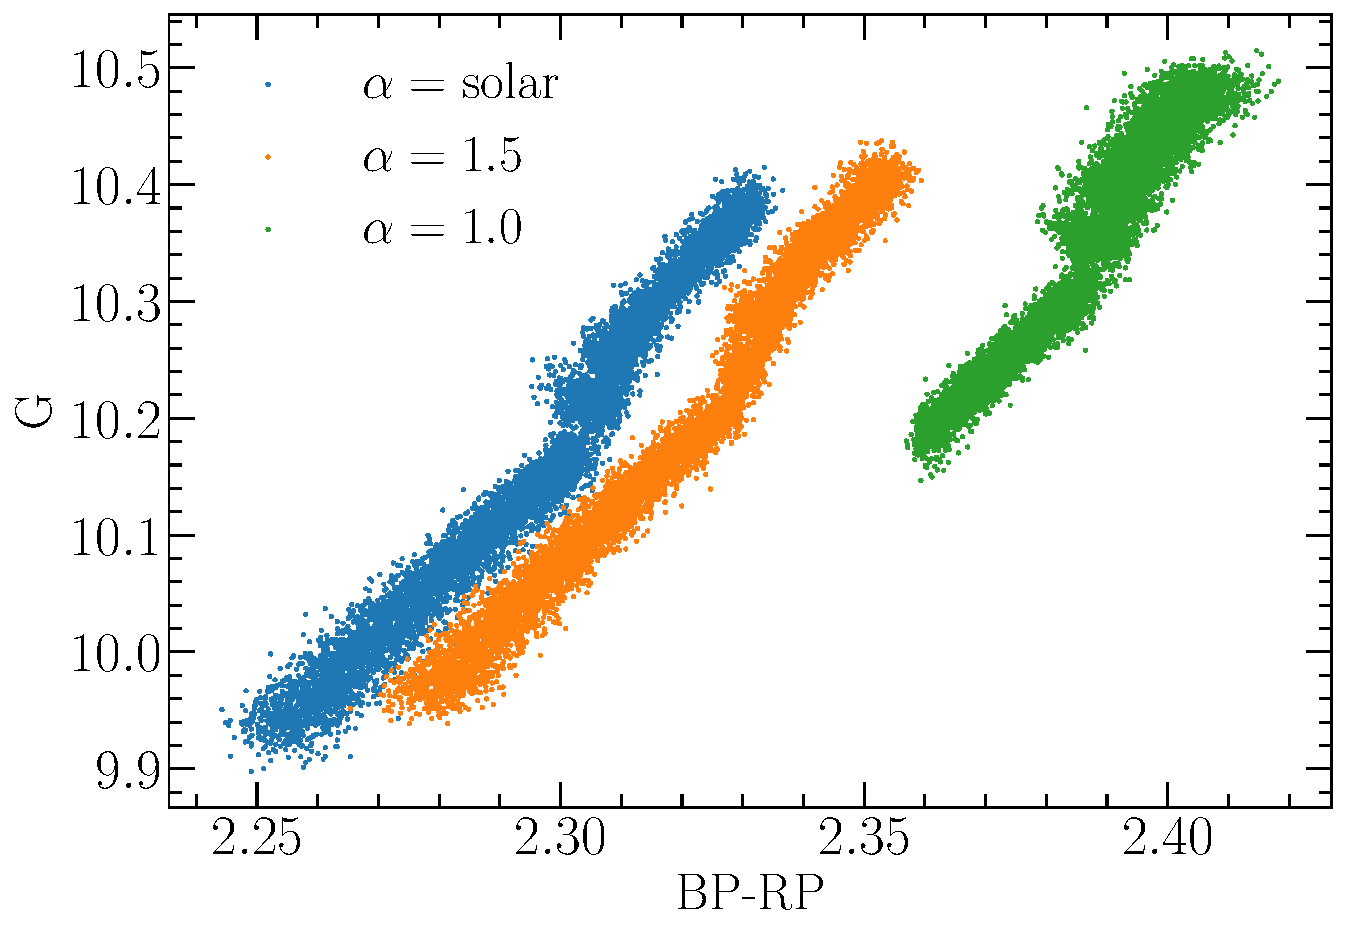
\includegraphics[width=0.8\textwidth]{./alphaMLComparisionCMD.pdf}
		\caption{Jao Gap seen in three populations using OPLIB high temperature
		opacities. From left to right these use a solar calibrated mixing length,
		a mixing length of 1.5, and a mixing length of 1.0}
		\label{fig:alphaMLCMD}
	\end{figure}
	\begin{figure}
		\centering
		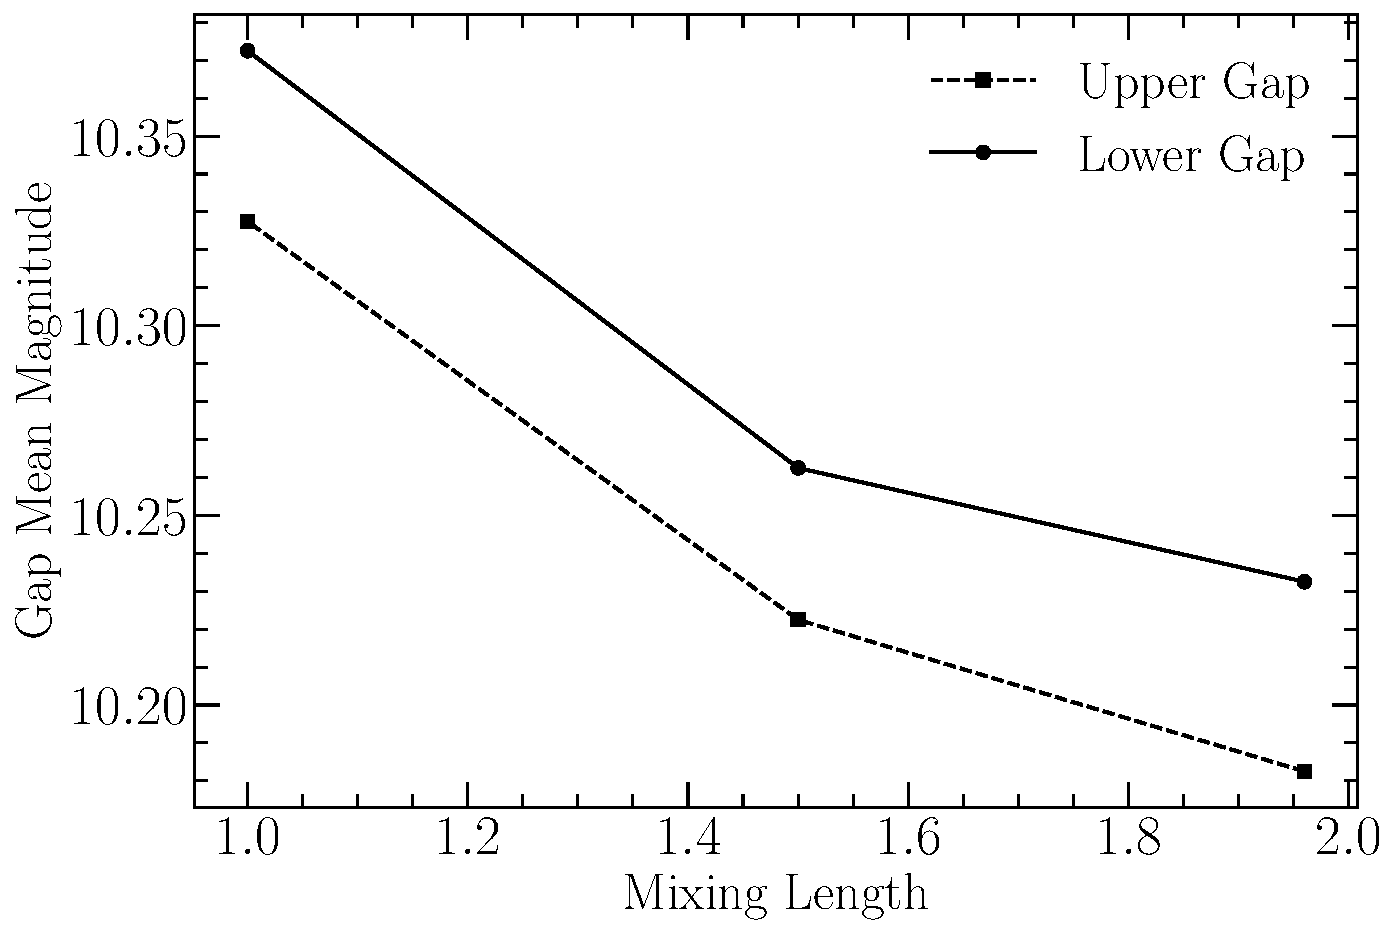
\includegraphics[width=0.8\textwidth]{./MixingLengthScaling.pdf}
		\caption{Identified locations of the two density dips we observe as a
		function of the Mixing Length used in those populations.}
		\label{fig:alphaMLLoc}
	\end{figure}
\end{reply}

\begin{point}
	On trying the web interface for the OPLIB, it seems that the process of
	interpolating between rho and R is unnecessary. Once T is specified, it is
	possible to get the same set of R values as for the OPAL tables by
	specifying the starting value of rho. Then only interpolation in T is
	needed to get a table in the same form as the OPAL tables. The authors need
	to clarify why they chose their approach. Also, it would be helpful to
	include in figure 15 a line plot of fractional difference against log T for
	log R = -1.5 or a different R value if -1.5 is not found to be
	representative for the radiative zone (see point 4). \label{pt:webR}
\end{point}

\begin{reply}
	The referee is correct that given a fixed temperature it is possible to
	extract specific R values from the OPLIB web form by specifying the correct
	density range. While we ultimately do not modify our querying program to
	operate like this we thank them for addressing this.

	We do not modify \texttt{pyTOPSScrape} as unfortunately this query method is
	not practically feasible when using a range of temperatures and densities
	simultaneously. Specifically, because each temperature within such a range
	would require a unique density range to be specified in order to match the
	OPAL table R range. This is not a feature offered by the webform.

	The reason we avoid querying a single temperature at a time is that making
	a separate call to the TOPS webform for not just each composition but also
	each temperature in that composition would increase the traffic per OPAL
	table by a factor of 70 (from 126 calls currently to 8820). This is both
	infeasible from a runtime perspective (as opening a new call is the most
	time intensive part of the scraper as the JavaScript engine is initialized
	and would likely push the generation time of a single table from 10
	minutes to over 5 hours) and would place a significantly increased load on
	the Los Alamos servers. We have spoken with the Los Alamos team and have
	their consent to release this software with only with the current traffic
	it generates. 

	A brief description of this has been included in Appendix B.

	The vertical line on Figure 13 has been updated to reflect the more accurate 
	approximation of Log(R) = -0.79 throughout the star as opposed to -1.5.
\end{reply}


\end{document}
